\documentclass{beamer}

\usetheme[iohk]{welltyped}
\usepackage{graphicx}
\graphicspath{ {../includes/} }

\begin{document}

\title{OPODIS PRESENTATION TITLE}
\subtitle{subtitle subtitle}
\author{Armando Santos}
\date{\today}
\maketitle

\AtBeginSection[]{
  \begin{frame}
  \vfill
  \centering
  \begin{beamercolorbox}[sep=8pt,center,shadow=true,rounded=true]{title}
    \usebeamerfont{title}\insertsectionhead\par%
  \end{beamercolorbox}
  \vfill
  \end{frame}
}

\begin{frame}{Table of Contents}
  \tableofcontents
\end{frame}

\section{Introduction}
\subsection*{Networking Team}
\begin{frame}{Networking Team}
  \begin{columns}
    \column{.33\linewidth}
    \centering
    Armando Santos \\ Well-Typed
    \column{.34\linewidth}
    \centering
    Marcin Szamotulski \\ Input Output Global
    \column{.33\linewidth}
    \centering
    Duncan Coutts \\ Well-Typed
  \end{columns}
  \vskip1cm
  \begin{columns}
    \column{.4\linewidth}
    \centering
    Neil Davies \\ PNSol
    \column{.4\linewidth}
    \centering
    Peter Thompson \\ PNSol
  \end{columns}
\end{frame}

\section{What we are doing}

\subsection*{Cardano Node}
\begin{frame}{Cardano Node}
\end{frame}

\subsection*{Decentralised Network}
\begin{frame}{Decentralised Network }
\end{frame}

\section{How we are doing it}

\subsection*{Functional Programming}

\begin{frame}{Functional Programming}
  Strongly Statically Typed Purely Functional Programming with \alert{Haskell}!

  \begin{itemize}
      \item Lazyness
      \item Type Safetiness
      \item Referential Transparency
      \item STM
      \item QuickCheck
      \item More!
  \end{itemize}

\end{frame}

\subsection*{Typed Protocols}

\begin{frame}{Typed Protocols}
  Internally developed (but open-source) library to specifyy end-to-end protocols at the type-level!

  \begin{itemize}
    \item Type Safe
    \item Session Types
    \item \alert{Deadlock free!}
    \item Pure
    \item Powerful (pipelining out of the box)
  \end{itemize}

\end{frame}

\subsection*{QuickCheck}

\begin{frame}{QuickCheck}
  Property based testing framework for Haskell.

  \begin{itemize}
    \item \alert{Input random generation}
    \item Shrinking
    \item \alert{Reproducibility}
    \item Coverage checks
  \end{itemize}

\end{frame}

\subsection*{IO Simulator}
\begin{frame}{IO Simulator}
  Simulation monad that is a drop-in \alert{replacement} for IO!

  Internally developed (but open source) library to perform all kinds of IO
  Simulations, in particular:

  \begin{itemize}
    \item write \alert{network simulations}, to verify a complex networking stack
    \item write {disk IO simulations}, to verify a database implementation
  \end{itemize}
\end{frame}

\subsubsection*{IO Simulator allows...}
\begin{frame}{IO Simulator allows...}
  \begin{columns}
    \begin{column}{0.4\textwidth}
      \begin{itemize}
        \item Early detection of critical races
        \item Simulation of rare \alert{edge cases}
        \item Mocking and \alert{error injection}
        \item Simulate time passing
        \item Looking for \alert{different schedules}
      \end{itemize}
      Most importantly:
      \begin{itemize}
        \item Allows for testing production code and
        \item Reproducing complex edge-case test failures
      \end{itemize}
    
    \end{column}
    \begin{column}{0.6\textwidth}
        %Content
      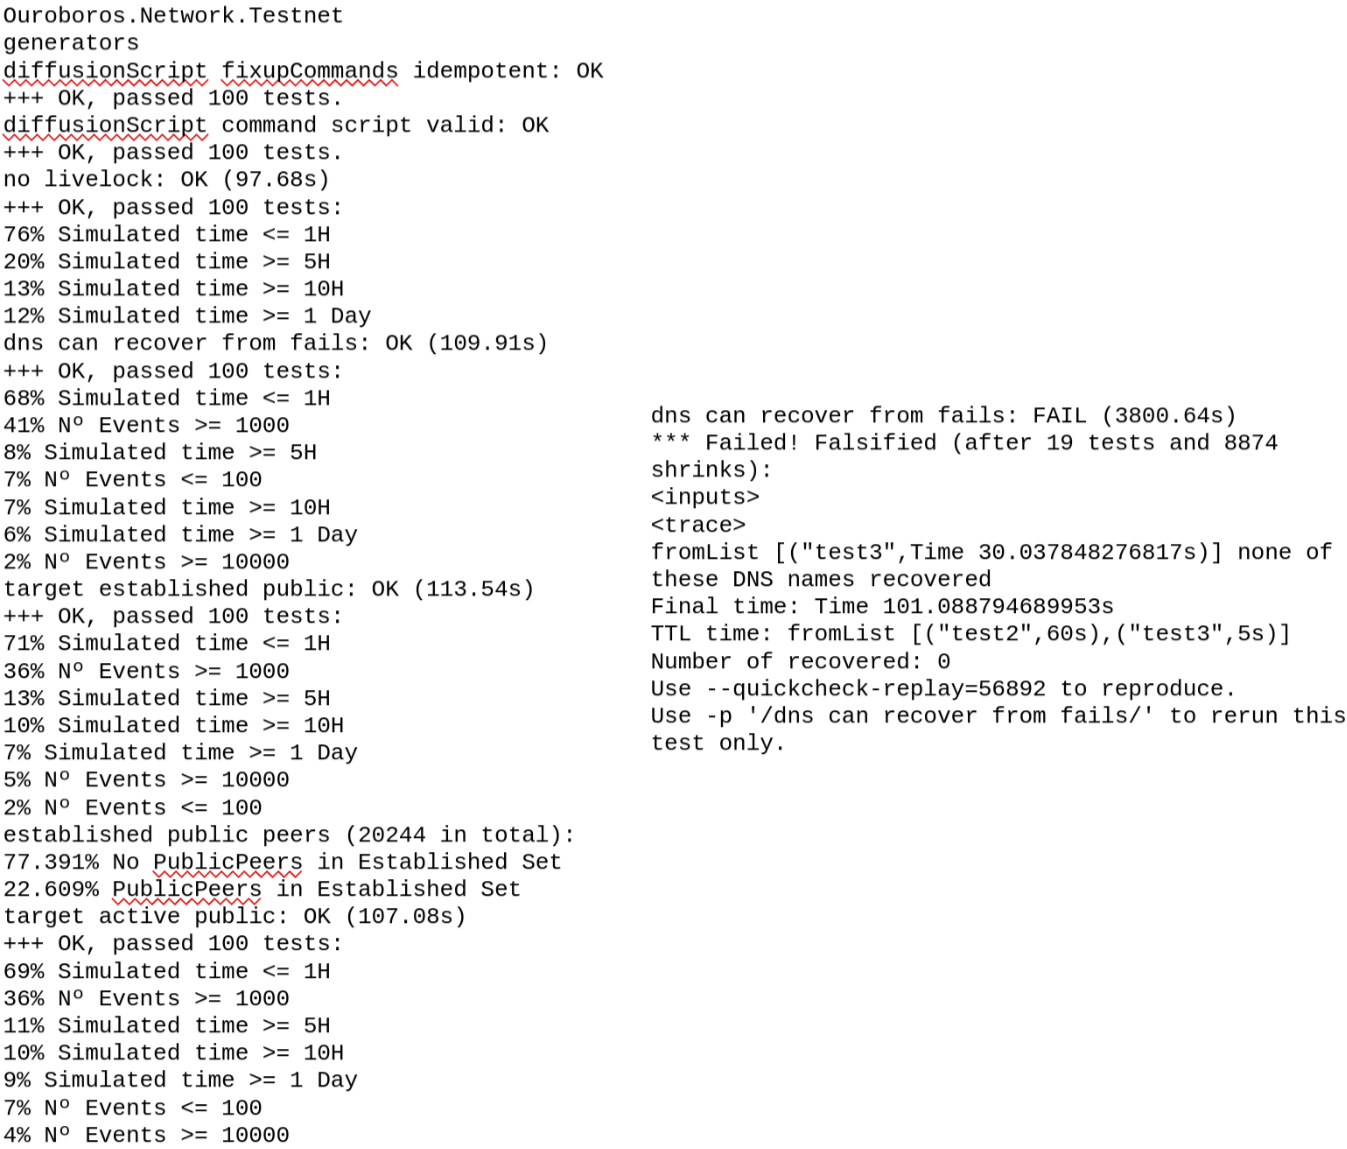
\includegraphics[scale=1.2, width=\textwidth]{code.png}
    \end{column}
  \end{columns}
\end{frame}

\section{What success looks like}

\section{Conclusion}

\end{document}

